\documentclass{article}
\usepackage{amsmath}
\usepackage{amsfonts}
\usepackage[utf8x]{inputenc}
\usepackage{default}
\usepackage[margin = 1in]{geometry}
\usepackage{natbib}
\usepackage{graphicx}
\usepackage{rotating}
\usepackage{wrapfig}
\usepackage[nolists]{endfloat}

\title{Conspicuous Consumption: Testing and Measurement using Household Budget
Surveys}
\author{David Jinkins}

\begin{document}
\maketitle

\section{Introduction}
Economists have long theorized about the role of conspicuous consumption in household spending decisions.  When a consumer decides which products to buy, part of her decision is based on what society will infer about her after observing what she chooses.  Introspection lends credence to this theory, but researchers have only recently attempted to measure the importance of conspicuous consumption in consumer demand.  
This paper uses household budget survey data to estimate a structural model of conspicuous consumption and consumer demand.  

In this research agenda, I take conspicuous consumption to be a mechanism for signaling wealth, or well-being.\footnote{It is important to note that this is different than signaling social status, to the extent that status is not perfectly correlated with wealth.  Also, the signal is not about relative wealth, but about absolute wealth, which differentiates this research from the ``positional goods'' literature associated with Cornell's Robert Frank.}  I am taking the point of view that the reason people consume conspicuous goods is that they can be at least partially observed by society, and inform society about the consumer's (unobservable) wealth.  There have been several recent empirical studies in this vein of research.  In one notable study, \citet{Blochetal2004} estimate a reduced form model of dowries and spending on wedding celebrations in India, and find results consistent with the idea that dowries buy the quality of husband (invisible), and weddings signal the status of husbands to society (conspicuous).  In a recent paper, \citet{Heffetz2011} conducts a telephone survey in the United States to determine the visibility of consumption goods.  Heffetz then analyzes household budget survey data, and finds evidence that the relitively visible goods identified by the survey are being used as a means to signal wealth. 

Since conspicuous consumption is a distortion from what would otherwise be an individual's optimal choice of goods, it is costly in terms of consumer welfare.  If people care deeply about social status, then the welfare cost of the distortion may be large.  Moreover, if everyone's wealth was known to society, then there would be no reason to overconsume conspicuous goods.  This point seems particularly poignant when considering the spending habits of the very poor.  A recent study reports that in parts of India, the \emph{median} household making under a dollar a day spends 10\% of its income on festivals--this while 43\% of such households did not have enough to eat throughout the year \citep{BanerjeeDuflo2007}.  Could it be that the poor overconsume festivals as a signal that they are not even poorer?  If so, there are policies such as taxing festival spending that may substantially increase welfare.  Measuring the importance of conspicuous consumption to consumers is a first step in gauging the social benefit of such a policy.

It is worthwhile to take a moment to differentiate the estimation of conspicuous consumption at hand from the relatively large literature on estimating interdependent preferences.  Beginning with James Duesenberry's 1949 doctoral thesis,\footnote{Later published as \citep{Duesenberry1949}} researchers have theorized that the consumption of neighbors affects own demand.  A typical econometric model in this literature lets household demand parameters depend linearly on the (weighted) average consumption of a reference group. A relationship between neighbor consumption and own consumption is taken to mean that preferences are interdependent.  The literature, however, does not take a stance on why consumption is interdependent, and it is hard to interpret what the estimated coefficients really mean.\footnote{To cite one of the first econometric papers in this literature, \citet{Pollak1976} speculates that exposure to the consumption of ``superior'' goods leads one to develop a taste for them.}  

Ori Heffetz and several others have provided reduced form evidence that conspicuous consumption may be important in explaining household purchasing behavior.
I expand on this literature by introducing a structural estimation of household utility which aims to explain just how strong this conspicuous consumption effect may be.
In addition, a fully specified model allows me to perform counter-factuals to guage the welfare benefits of taxing conspicuous good.
\footnote{This model is very partial equilibrium, however, taking prices as given and totally extracting away from the production side of the economy.}

\section{Environment}
There is a continuum of consumers who live for a single period and are endowed with an exogenous wealth level $w \in \left[ \underline{w},\overline{w} \right]$.
Consumers use this wealth to buy goods with exogenous prices $\{p_i\}_I$ in order to maximize a utility function on the space of good categories $I$, $\|I\|<\infty$. 
Consumers vary in wealth level, which is observable to the econometrician, and preference type, which is not observable.
Preference types $\gamma$ is a vector of length $\|I\|$ and are drawn from a distribution $G$.

The utility function consists of two parts.  The first part is a fundamental utility $u:\mathbb{R}_+^{\|I\|}\rightarrow\mathbb{R}$.
The fundamental utility describes the pleasure consumers get directly from consuming a bundle of goods.
The second part is a social belief over an consumer's utility.  
Society is a passive actor who forms a belief over an consumer's utility level after observing the expenditure of the individual on a single good category. 
There are two versions of the model.
In the first version, the individual does not know which good society will observe. 
Consumption decisions are made before this uncertainty is resolved.
Probabilities of observation are weighted by the visibility of a good.
In the second version, society announces which good it will be observing before the consumer chooses makes his consumption decision. 
Again, the good which society announces to the consumer is chosen randomly, weighted by the visibility of the good categories.
Although the timing of the first version is more plausible, the second version allows me to base inference on preference heterogeneity.
\footnote{The timing in the second version can be justified by trends in circles of friends.  This year, many of my friends bought tablet computers.  This year then, socieities guess about my well-being might depend upon my spending on electronics.  In another year, clothing might be more important.  The key point is that I know what the trend is before I make my consumption decisions.} 
In addition, the second version gives me closed form results for equilibrium consumption, which greatly simplifies the estimation.
In the first version, I shut down preference heterogeneity and assume that the variation in consumption decisions of the same wealth type is due to measurement error.
Currently I am concentrating on the second version.

In both versions of the model, there is a category-dependent social belief functions mapping consumption to wealth level, $W:I\times[0,\infty]\rightarrow[0,\infty]$.
In the first version of the model, there is a single vector valued function mapping wealth level to consumption, $\hat{C}:[0,\infty]\rightarrow [0,\infty]^{\|I\|}$.
In the second version, the consumption map depends on the good category announced to the consumer, $\hat{C}:I\times[0,\infty]\rightarrow [0,\infty]^{\|I\|}$.
Note that preference type does not appear in the consumption map.
This is because in the first version of the model I assume preference homogeneity, and in the second version I assume that society assigns the consumer the (half-space) median preference value, which in my specialization will be equivalent to the modal preference value.
\footnote{The half-space or Tukey median is a generalization of median to multi-dimensional distributions.  Each point on the support of a probability distribution is assigned a depth, which is defined as the smallest measure of a half-space containing the point. The half-space median is defined as the set of points with the maximum depth.  Note that for a uni-variate distribution, this definition coincides with the set of median values. This concept was introduced by Tukey (1975), a paper that is also distinguished by beginning with the sentence: 'Why am I writing on this topic?'}
In other words, society assumes that any particular person is typical in preference value.

Consumers care about what society believes about their wealth level, so this social belief enters as a second term in the utility function.
Following earlier literature (Heffetz,Ireland) I assume the utility function is additively separable in fundamental utility and social belief.
In the first version of the model, the total utility function is written: \[U(C) = (1-\alpha) u(C) + \alpha \sum_1^{\|I\|} v_i u(\hat{C}(W(i,c_i)).\]
Here $v_i$ is the visibility weighted probability of observation.
In the second version of the model, the utility function is written:
\[U(C,\gamma,i) = (1-\alpha) u(C,\gamma) + \alpha\  u(\hat{C}(i,W(i,c_i)),\overline{\gamma}).\]
Note that society assigns the median $\gamma$ to every consumer.  
\subsection{Equilibrium Concept}
Let $r$ be an exogenous vector of prices.  
To simply notation, define the composite social belief function $\mathcal{C}(i,c_i)=\hat{C}(i,W(i,c_i))$. 
%Given the social belief function, the problem for a consumer of wealth type $\tilde{W}$ in the first version is:
%\[ \max_C \ U(C) :  r\cdot C \le \tilde{W}\]
%An equilibrium is a composite social belief function $\mathcal{C}$  and a function $\tilde{C}$ on wealth such that:
%\begin{enumerate}
%	\item $\forall \tilde{W}, \tilde{C}(\tilde{W})$ solves the consumer's problem for wealth type $\tilde{W}$.
%	\item $\forall (\tilde{W},i), \ \mathcal{C}(i,\tilde{C}_i(\tilde{W})) = \tilde{C}(\tilde{W}).$
%\end{enumerate}
%
The consumer's problem in the second version of the model for a consumer of wealth type $\tilde{W}$, preference type $\gamma$, and announced good $i$ is:
\[ \max_C \ U(C,\gamma,i) :  r\cdot C \le \tilde{W}\]
An equilibrium is a composite social belief function $\mathcal{C}$ and a consumption function on $(\tilde{W},\overline{\gamma},i)$ such that:
\begin{enumerate}
	\item $\forall (\tilde{W},i), \ \tilde{C}(\tilde{W},\overline{\gamma},i)$ solves the consumer's problem for type $(\tilde{W},\overline{\gamma},i)$.
	\item $\forall (\tilde{W},i), \ \mathcal{C}(i,\tilde{C}_i(\tilde{W},\overline{\gamma},i)) = \tilde{C}(\tilde{W},\overline{\gamma},i).$
\end{enumerate}
Here $\tilde{C}_i(\tilde{W},\overline{\gamma},i)$ refers to the $i$-th element of the vector $\tilde{C}(\tilde{W},\overline{\gamma},i)$.
The first condition says that all consumers choose an optimizing  bundle, and the second condition says that society is able to completely learn the well-being of each consumer, regardless of the consumer's observation type.
The equilibrium conditions need only apply to consumers of preference type $\overline{\gamma}$, since society assumes that any observed consumer is of this preference type.   
\subsection{Specializing to Stone-Geary}
Everything to the end of this note for now refers to the second version of the model presented above.  
Let the fundamental utility function be Stone-Geary:
\[u(C,\gamma) = \sum_{i=1}^{\|I\|} \beta_i \ln(c_i - \gamma_i - \psi_i))\]

Once the observation type is revealed there is no longer any uncertainty in the consumer's problem.
The model becomes a generalization of the Heffetz model to many goods and preference heterogeneity.\footnote{ In the Heffetz version, there are only two goods, one visible and the other invisible to society. In my version, there is one visible good for each observation type, and all the other goods are invisible.}
Let the median of the $G$ distribution be a vector of zeros, so that for the purposes of finding equilibrium we can ignore $\gamma$.

Let $v\in I$ be the observation type.
Suppose that $c_v^*$ is the equilibrium consumption of the visible good.
Then the consumptions of the other goods must satisfy:
\[ U(C^*,\bar{\gamma},v|c_v^*)=\underset{\{c_i\}_{i\neq v}}{\max} \ U(C,\bar{\gamma},v|c_v^*) :  \sum_{i \neq v} r_i c_i \le W-r_v c_v^*\]
Assuming that all of the $\psi_i$ are non-negative, we can write the equilibrium consumption for any good $i\neq v$ as:
\[ c_i^* = \psi_i + \frac{\beta_i}{r_i}\left(\sum_{j\neq v} \beta_j\right)^{-1}\left(W-r_v c_v^* - \sum_{j\neq v} r_j \psi_j\right)\]
Plugging these demands into the equilibrium utility function we get:
\begin{align}
	U(C^*,\bar{\gamma},v) &= (1-\alpha)\sum_{i\neq v} \beta_i \ln\left(\frac{\beta_i}{r_i}\left(\sum_{j\neq v} \beta_j\right)^{-1}\left(W-r_v c_v^* - \sum_{j\neq v} r_j \psi_j\right)\right) + h(c_v^*) \nonumber \\ 
	&= (1-\alpha) \ln\left(\prod_{j\neq v} \left(\frac{\beta_j}{r_j}\right)^{\beta_j}\left(\sum_{j\neq v} \beta_j\right)^{-\sum_{j\neq v} \beta_j}\left(W-r_v c_v^* - \sum_{j\neq v} r_j \psi_j\right)^{\sum_{j\neq v} \beta_j}\right) + h(c_v^*) \nonumber \\ 
	\label{invop}
	&= (1-\alpha) \hat{\beta} \ln \left(W-r_v c_v^*-\hat{\psi}\right) + h(c_v^*) + \hat{\zeta} 
\end{align}
Here $h(c_v^*)$ is the part of the utility function which does not depend upon any of the invisible goods, and:
\begin{align*}
	\hat{\beta} &= \sum_{j\neq v} \beta_j\\
	\hat{\psi} &= \sum_{j\neq v} r_j \psi_j\\
	\hat{\zeta} & = (1-\alpha) \ln\left(\prod_{j\neq v} \left(\frac{\beta_j}{r_j}\right)^{\beta_j}\left(\sum_{j\neq v} \beta_j\right)^{-\sum_{j\neq v} \beta_j}\right) 
\end{align*}

Society knows that given wealth and the consumption of the visible good, it is optimal to split consumption among the invisible goods as derived above.  Thus using \eqref{invop}, we can rewrite the total utility function as: 
\[U(C,\bar{\gamma},v) = (1-\alpha) \left(\hat{\beta} \ln \left(W-r_v c_v-\hat{\psi}\right) + \beta_v \ln \left(c_v - \psi_v\right)\right) + \alpha \left(\hat{\beta} \ln \left(g(c_v) - \hat{\psi}\right) + \beta_v \ln \left(c_v - \psi_v \right) \right) + \hat{\zeta}\]
Here $g(c_v)$ is society's guess about $W-r_v c_v$ based on $c_v$. 
In particular, note that society's belief over a consumer's utility is described by a single-dimensional function.

The first order conditions for an interior solution to the consumer's problem can be written:
\begin{equation}
g'(c_v) = \frac{1}{\alpha}\left( \left( 1-\alpha\right) r_v - \frac{\beta_v}{\hat{\beta}}\frac{g(c_v)-\hat{\psi}}{c_v - \psi_v}\right)
\end{equation}

Now we can directly follow Heffetz and solve this differential equation:
\begin{equation}
	\label{difsol}
	g(c_v) - \hat{\psi} = \frac{\hat{\beta}\left(1-\alpha\right)}{\beta_v +\alpha \hat{\beta}} \left(c_v-\psi_v\right) + K\left(c_v-\psi_v\right)^{\frac{\beta_v}{\alpha \hat{\beta}}}
\end{equation}
To solve for the constant $K$, note that the lowest wealth type $\underbar{W}$ has no reason to signal in a separating equilibrium.
In particular, his consumption will not be distorted, so that his demand for $c_v$ will be given by:
\[
c_v^* = \psi_v + \frac{\beta_v}{r_v}\left(\sum_{j} \beta_j\right)^{-1}\left(\underbar{W} - \sum_{j} r_j \psi_j\right)
\]
Since in equilibrium $g(c_v^*) = \underbar{W} - c_v^*$, we can plug into \eqref{difsol} and solve for $K$.
This part of the analysis directly follows from Heffetz.
\section{Data}
This project requires three types of data.  We need consumer expenditure data at the household level, we need relative price data, and we need demographicly differentiated information about how visible different good categories are relative to each other. 
\subsection{Vindex data}
Data about the relative  conspicuousness of  various types of goods is taken from Heffetz.  
Heffetz bases the index on randomized telephone surveys conducted in the United States in several waves around 2004.
The main questions of interest were about good categories.
Heffetz asked respondents how long it would take them to notice if a new acquaintance similar to themselves spent more than average on a particular good category.
Repondents were able to choose from five time periods ranging from almost immediately to almost never.  
Basic demographics were also recorded for respondents.  

Heffetz create indexes (called vindexes) between zero and one for each category of goods by averaging over survey results.  
A higher index implies that a good category is  more conspicuous. 
A result of this aggregation methodology is that the index is cardinal rather than ordinal.  Two goods with similar index values are similar in visibility.  Details on the implementation of the survey and calculation of the index are available in Heffetz (???).
Table \ref{tab:vintab} below is an example of a vindex table for non-blacks under 40.

\begin{table}
	\begin{center}
\begin{tabular}{|l|c|c|}
	\hline
Clo (clothing) & 0.78 & (0.02)\\ 
	\hline
Cig (cigarettes) & 0.75 & (0.02)\\ 
	\hline
Car (cars) & 0.72 & (0.02)\\ 
	\hline
Fur (furniture) & 0.69 & (0.02)\\ 
	\hline
Ot1 (recreation 1) & 0.68 & (0.02)\\ 
	\hline
Jwl (jewelry) & 0.68 & (0.03)\\ 
	\hline
FdO (food out) & 0.67 & (0.02)\\ 
	\hline
AlH (alcohol home) & 0.66 & (0.03)\\ 
	\hline
AlO (alcohol out) & 0.65 & (0.02)\\ 
	\hline
Ot2 (recreation 2) & 0.61 & (0.02)\\ 
	\hline
Brb (barbers etc) & 0.6 & (0.03)\\ 
	\hline
Bks (books etc) & 0.58 & (0.02)\\ 
	\hline
Edu (education) & 0.55 & (0.03)\\ 
	\hline
Hom (rent/home) & 0.54 & (0.03)\\ 
	\hline
FdH (food home) & 0.51 & (0.03)\\ 
	\hline
Cel (cell phone) & 0.47 & (0.03)\\ 
	\hline
Htl (hotels etc) & 0.46 & (0.02)\\ 
	\hline
Air (air travel) & 0.44 & (0.03)\\ 
	\hline
Bus (public trans.) & 0.44 & (0.03)\\ 
	\hline
CMn (car repair) & 0.38 & (0.03)\\ 
	\hline
Cha (charities) & 0.36 & (0.03)\\ 
	\hline
Gas (gasoline) & 0.34 & (0.03)\\ 
	\hline
Lry (laundry) & 0.32 & (0.03)\\ 
	\hline
Med (health care) & 0.32 & (0.02)\\ 
	\hline
Tel (home phone) & 0.25 & (0.03)\\ 
	\hline
Utl (home utilities) & 0.25 & (0.03)\\ 
	\hline
Fee (legal fees) & 0.24 & (0.02)\\ 
	\hline
CIn (car insur.) & 0.22 & (0.03)\\ 
	\hline
LIn (life insur.) & 0.15 & (0.02)\\ 
	\hline
Und (underwear) & 0.14 & (0.02)\\ 
	\hline
HIn (home insur.) & 0.13 & (0.02)\\ 
	\hline
\end{tabular}
\end{center}
\label{tab:vintab}
\caption{Vindex for non-blacks under 40.}
\vspace{-2in}
\end{table}
\subsection{Household Expenditure Data}
Household consumption expenditure survey  data is from the National Bureau of Economic Research website.    
This dataset is publically available, and features a random sample of American household consumption decisions for selected years between 1981 and 2002, with 18 years available all together.  
The dataset is based on more detailed and proprietary dataset collection by the United States Department of Labor. 
In addition to household expenditures, the NBER dataset contains some demographic data on household members such as age, race, sex, and location of the interviewee.  
\footnote{I reexamined the dataset today and found a region variable that I didn't know about.  The next step in the project is to code this into the estimation.}
There are 47 consumption categories available in the NBER data set.
Following Heffetz exactly (actually even using his code), I aggregate (and drop some inconsequential categories) into 29 categories used in the vindex.
All together, the my dataset contains 160,617 household interviews.
This number is so high that I have trouble looping through the whole dataset when I maximize the likelihood (details below)!

To give the reader some idea about what the data look like, I have chopped up the data a bit and included a couple of figures.  
In Figure \ref{fig:shr}, I scatter plot the log budget shares by log expenditures, and in Figure \ref{fig:lev} I scatter plot log category expenditures by log expenditures.  
I also included a histogram of log expenditures in Figure \ref{fig:exphist}.  
All of these plots are using only one year of the data (2001), just to keep the number of points in the scatter plots managable. 
The point I want to emphasize about these plots is that they are very noisy.
If we were to take the naive Heffetz or Ireland model at face value, all consumers of the same expenditure level should make the same consumption decisions.
\footnote{To be fair, Heffetz goes to great lengths in his paper to make this same point.  There is more than just two-good conspicuous consumption going on in the expenditure data.}
By adding 29 latent observation types and preference heterogeneity, the version of the Heffetz model estimated in this paper has a hope of matching this sort of noisy data.

\begin{figure}
	\begin{center}
		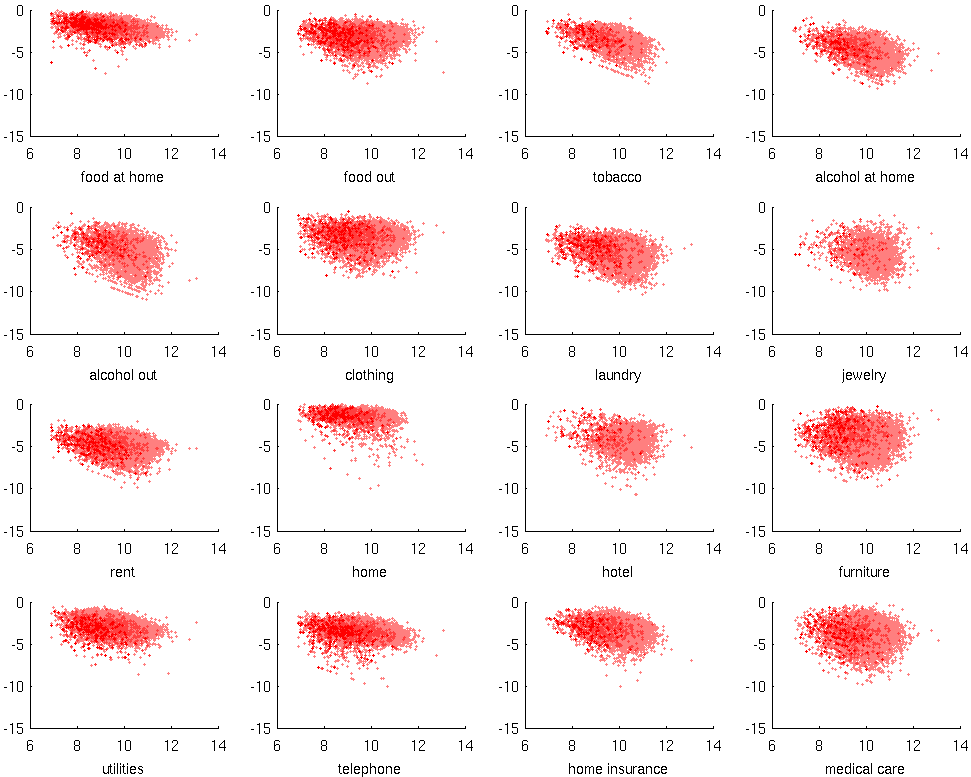
\includegraphics[scale=.8]{pics/shares_cropped.pdf}
	\end{center}
	\label{fig:shr}
	\caption{Log Expenditure Shares by Log Expenditure for select goods}
\end{figure}
\begin{figure}
	\begin{center}
		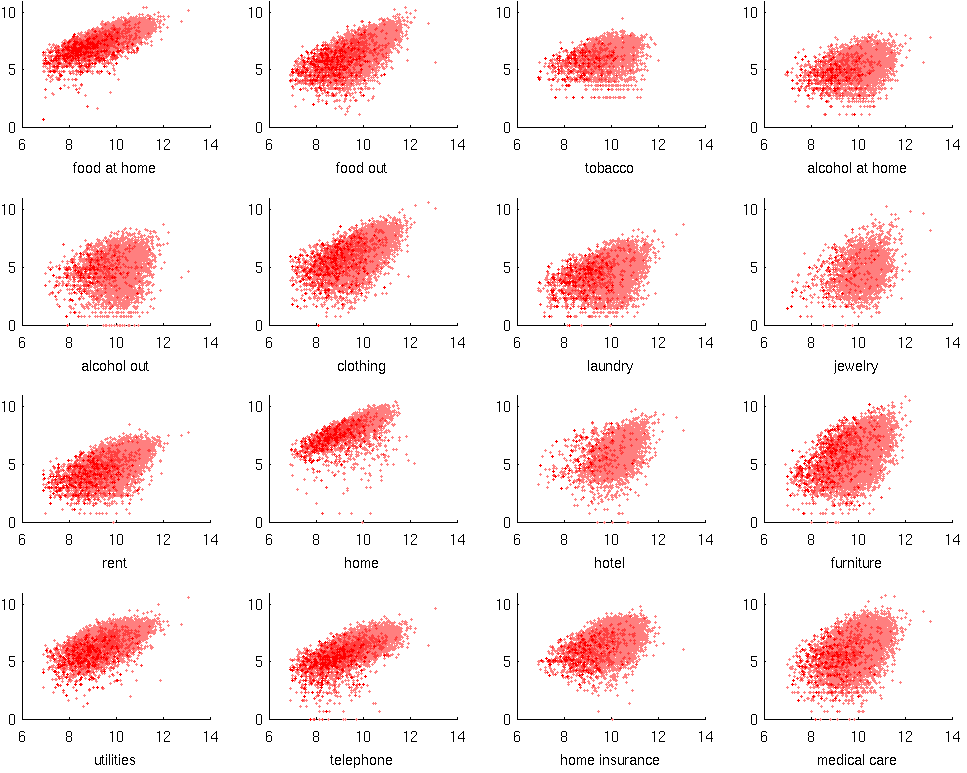
\includegraphics[scale=.8]{pics/levels_cropped.pdf}
	\end{center}
	\label{fig:lev}
	\caption{Log Category Expenditure by Log Expenditure for select goods}
\end{figure}
\begin{figure}
	\begin{center}
		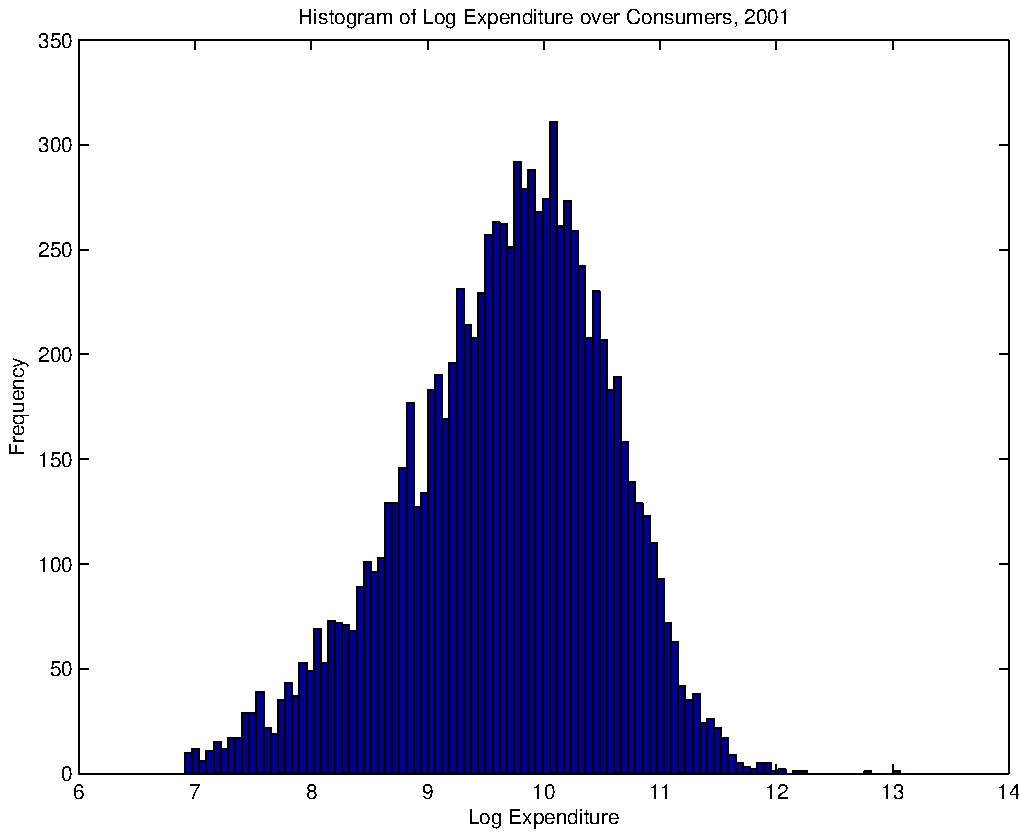
\includegraphics[scale=.8]{pics/exphist_cropped.pdf}
	\end{center}
	\label{fig:exphist}
	\caption{Histogram of  Log Expenditure}
\end{figure}
\subsection{Price Data}
I have a time-series of relative price data from the Bureau of Labor services.
Most of the NBER household consumption categories were easy to match with the definitions used by the BLS.   
Since prices are normalized to one in 1983, the units of each good which enter into the utility function are whatever one dollar could buy in 1983.
The following page is a table showing the price category names I used compared with the NBER consumption categories:

\begin{sideways}
\begin{tabular}{|l|l|l|}
\hline
VinCat Abrev & Vindex Category & PriceCatName\\ 
\hline
Brb & barbershops, beauty parlors, hair dresser, health clubs, etc. & Personal Care Services\\ 
\hline
Clo & clothing and shoes, not including underwear, undergarments and nightwear & Apparel\\ 
\hline
Cig & tobacco products like cigarettes, cigars, and pipe tobacco & Tobacco and Smoking Products\\ 
\hline
Jwl & jewelry and watches & Jewelry and watches\\ 
\hline
Car & the purchase of new and used motor vehicles such as cars, trucks, and vans & New and used motor vehicles\\ 
\hline
FdO & dining out at restaurants, drive-thrus, etc, exl. Alcohol incl. Food at school & Food away from home\\ 
\hline
Ot1 & computers, games, TVs, video, audio, musical and sports equipment, tapes, CDs. & Televisions\\ 
\hline
FdH & food and nonalcoholic beverages at grocery, specialty and convenience stores. & Food at home\\ 
\hline
Edu & education, from nursery to college, like tuition and other school expenses. & Tuition, other school fees, and childcare\\ 
\hline
Cel & mobile phone services. & Wireless Telephone Services\\ 
\hline
AlO & alcoholic beverages at restaurants, bars, cafeterias, cafes, etc. & Alcoholic Beverages away from home\\ 
\hline
AlH & alcoholic beverages for home use. & Alcoholic Beverages at home\\ 
\hline
Fur & home furnishings and household items, like furniture, appliances, tools, linen. & Furniture and bedding\\ 
\hline
Ot2 & cable TV, pets and veterinarians, sports, country clubs, movies, and concerts. & Cable and satellite television\\ 
\hline
Bks & books incl. School books, newspapers and magazines, toys, games, and hobbies. & Recreational reading materials\\ 
\hline
Cmn & vehicle maintenance, mechanical and electrical repair and replacement. & Motor vehicle maintainance\\ 
\hline
Hom & rent, or mortgage, or purchase, of housing & Housing\\ 
\hline
Htl & lodging away from home on trips, and housing for someone away at school. & other lodging away from home\\ 
\hline
Bus & public transportation, both local and long distance, like busses and trains. & Public transportation\\ 
\hline
Air & airline fares for out-of-town trips. & Airline Fare\\ 
\hline
Gas & gasoline and diesel fuel for motor vehicles. & Motor Fuel\\ 
\hline
Tel & home telephone services, not including mobile phones. & Telephone Services\\ 
\hline
Cha & contributions to churches or other religious organizations, and other charities. & Missing\\ 
\hline
Lry & laundry and dry cleaning. & Laundry equipment\\ 
\hline
Utl & home utilities such as electricity, gas, and water, garbage collection. & Fuel and Utilities\\ 
\hline
Med & medical care, incl. Health insurance, drugs, dentists, doctors, hospitals, etc. & Medical care\\ 
\hline
Fee & legal fees, accounting fees, and occupational expenses like tools and licenses. & Professional services\\ 
\hline
Cin & vehicle insurance, like insurance for cars, trucks, and vans. & Motor vehicle insurance\\ 
\hline
Hin & homeowners insurance, fire insurance, and property insurance. & Tenants' and household insurance\\ 
\hline
Lin & life insurance, endowment, annuities, and other death-benefits insurance. & Health insurance\\ 
\hline
\end{tabular}
\end{sideways}

\section{Derivation of Estimation Equations}
The strategy in this section is to use maximum likelihood to estimate the parameters of the model.  
While there is no uncertainty in the model for consumers, their are two parameter sets that are unobserved by the econometrician.
The first is a latent variable--the announced observation type.
The second is preference heterogeneity.
As is standard in this type of problem, I proceed with the EM algorithm.
In the first step, I randomly assign each household an announced observation type.
Then I get parameters by maximizing the likelihood with respect to preference heterogeneity.
Next I use the model parameters to assign the observation types with the highest likelihood.
Using these observation types, I get a new set of parameters using maximum likelihood over the preference heterogeneity.
This process is repeated until there is no reassignment of observation type.

The first order of business is to derive the likelihood function.
As a reminder, the utility function now looks like this:
\begin{equation}
	\label{totuti}
U(C,\gamma,v) = (1-\alpha) \sum_{j=1}^{29}\beta_j \ln(c_j - (\psi_j+\gamma_j))  + \alpha \left(\beta_v \ln(c_v - \psi_v)+ \hat{\beta}\ln(g(c_v,v) - \hat{\psi}) + \hat{\zeta} \right)
\end{equation}
In the literature, the heterogeneity in linear expenditure systems is usually put on the $\beta$ terms (pitt and lee, for example).
The reason I put the heterogeneity on the $\psi$ term has to do with zeros in my data.
Some households report zero spending in consumption categories (charitable spending, for instance, is rather sparce).
If I were to put the heterogeneity on the $\beta$, then to explain the zeros nearly all the $\psi$ terms would have to be negative.
This situation is undesirable, however, as the theoretical results I derived above require all of the $\psi$ to be positive (for the typical consumer).
Putting heterogeneity on the $\psi$ terms allows me to both explain zeros in the data, and use the convenient theoretical results above.
The cost of this strategy is that there is no closed for solution to the Stone-Geary demand system when $\psi$ is negative.
 Using the standard formula given above would imply negative consumption for highly negative values of $\psi$.

 This notwithstanding, for now I am going to use the standard formula anyway, and assume that it is rare to get a value of $\psi$ so negative as to cause negative consumption.
 Of course, in the data, there is no negative expenditure.
 What I am assuming here is tantamount to saying that if a consumer has zero expenditure in some good category, then if her preference shock would have been a little more negative, she would have had negative consumption.
 This assumption is not too far-fetched if the shock variance is relatively small given that I will assume the shocks follow a normal distribution (the exponential tails die quickly).\footnote{The other side of the coin is also possible--if the $\psi$ is too positive, then a consumer dies, and doesn't appear in the data.  Again I assume this is rare enough to ignore it.}
I assume that the preference shocks $\gamma$ are distributed independent normal $\mathcal{N}(0,\sigma_i)$.
This implies a median vector of zeros as desired.

Consider a household of wealth type $W$ and with consumption vector $C$.  
Suppose that the household is observation type $v$.
Then the consumptions of goods $j\neq v$ are given by:
\begin{equation}
	\label{eq:sgd}
	r_jc_j = r_j(\psi_j + \gamma_j) + \frac{\beta_j}{\sum_{i\neq v}\beta_i}  \left(W-\sum_{i \neq v} r_i\left(\psi_i + \gamma_i\right) - r_v c_v\right).
\end{equation}
Note that \eqref{eq:sgd} can be written as a system of 28 linear equations, which can be easily solved (even by hand, although this would be ugly).
Once we have solved for the gammas, we can calculate a likelihood for each announced observation type possibility.
Of course, we are still missing $\gamma_v$ from the good which society observes.
$\gamma_v$ can be approximated by using the implicit function theorem and a Taylor expansion around the median preference type's optimal consumption $c_v^*$ in \eqref{totuti}:
\begin{equation}
	\frac{\partial \psi_v}{\partial c_v}|c_v^* = \frac{1}{\frac{\partial c_v}{\partial \psi_v}}|c_v^*=\frac{\alpha \hat{\beta}}{\beta_v}\left(c_v^*-\psi_v\right)^2 \left( \frac{g'(c_v^*)}{g(c_v^*)-\hat{\psi}} - \frac{g^{''}(c_v^*)}{\left(g(c_v^*) -\hat{\psi}\right)^2}-\frac{r_v}{\alpha \hat{\beta}(W-\sum_{j\neq v} r_j (\psi_j + \gamma_j) -r_v c_v^*)^2}\right)
\end{equation}
The approximation is then:
\begin{equation}
	\gamma_v \approx \left(\frac{\partial \psi_v}{\partial c_v}|c_v^*\right)\left(c_v - c_v^*\right)
\end{equation}
It should be noted that to get the $g$ function, I need to estimate the lowest social wealth level. 
At first blush, it appears that using the minimum wealth level in my data set would be a good estimator for this wealth level.
Presumably due to measurement error, however, the data set contains a few unbelievably low values--the lowest (positive) value is something on the order of six dollars of annual expenditure.
In practice, I assume the lowest possible wealth level is one thousand dollars, and drop any households with lower expenditure.
Out of my 160,617 household observations, 4722 are dropped.
The dropped observations include something like 2500 observations which have negative annual expenditures, caused by reported negative consumption (NEED TO CHECK EXACT NUMBER).
For completeness, given an observation type $v$, the likelihood function for a particular household is written as follows:
\begin{equation}
	\label{lik1}
	l(v,W,C,\theta) = \sum_{j} \ln \phi(\gamma_j,0,\sigma_j)
\end{equation}

Up to this point, I have not introduced the Heffetz vindex into the estimation. The vindex enters in the next step (the E step in the EM algorithm).
Given a set of parameters, we need to choose the most likely observation types.
This calculation is as follows:
\begin{equation}
	pr(i|W,C,\theta) = \frac{v_i l(i,W,C,\theta)}{\sum_j v_j l(j,W,C,\theta)}
\end{equation}
  The $v_i$ here is the vindex probability, or the probability of society choosing that particular good to announce.
In practice I have different visibility indexes for four groups of households: blacks under 40, blacks over 40, non-blacks under 40, and non-blacks over 40.
\footnote{A household is identified by the self-identified characteristics of whoever answered the consumption survey.} 
The visibility probabilities are taken directly from Heffetz and normalized so that they sum to one.
\footnote{In a previous version of this project, I needed to calculate equilibrium consumptions for each type.  This led me to keep the type nmber small.  In the current version, the fineness of the type does not affect the speed of estimation.  One of the next things on the plate, in terms of this project, is including very fine types--as fine as allowed by the Heffetz survey.}

The vector $\theta$ of parameters to be estimated contains 59 utility function parameters and 29 standard deviations for the preference heterogeneity.  
This totals to 88 parameters.  
However, since the preference heterogeneity is assumed to be independent normal, the sample variance in the $\gamma$'s gives me the likelihood maximizing value for the $\sigma$'s.
Thus I have only the 59 utility parameters to estimate in the EM loop. 
In my useable dataset, I have 155,270 households which is more than 2,500 household observations per parameter.
\section{Discussion of Estimation}
I am currently using only 10,000 randomly chosen household observations in the EM algorithm.
When I impliment parallel computing in the code, I should be able to handle all of the data at about the same speed (since I have access to 12 cores to run at any given time).
The likelihood algorithm needs to loop over household observations.
The reason I haven't been able to just change the for to parfor in the code is that the task per observation is very quick, only a fraction of a second.
The overhead of passing information back and forth between cores with such quick tasks makes is quicker to just use a standard serial process.
The typical way to solve this problem is to group the small tasks into larger tasks to be passed to individual cores.  
In any case, this is probably the next thing I will implement in the code.

With 10,000 observations, it takes about two seconds to evaluate the likelihood function once.
Since the solver I am using (knitro) needs to approximate the jacobian at each iteration, one iteration of the likelihood solver takes about two minutes.
The second step in which the most likely observation types are chosen takes a bit longer to run one iteration, but usually only needs to run onc or two iterations before the EM algorithm converges stops.

One issue is the appearance of NaNs and infs in the likelihood estimation. 
This happens occasionally, and rather than kill the loop I currently just penalize the likelihood.
I do this by adding a log likelihood value about ten times worse than the minimum of likelihood values appearing in a typical run.
The infs appear when the likelihood is very low, so that MATLAB approximates with zero.
I haven't been able to diagnose the occassional NaN yet.

\section{Preliminary Results}
\bibliographystyle{plainnat}
\bibliography{biglist.bib}
\end{document}
